\documentclass{article}

\usepackage{hyperref}
\usepackage{graphicx}
\usepackage{pdflscape}
\usepackage{pdfpages}


\title{Distributed Artificial Intelligence \\ \large{Report Assignment 5/Lab 8}}
\author{Ewout Pockelé \\ \href{mailto:ewout.pockele@student.uantwerpen.be}{ewout.pockele@student.uantwerpen.be}}


%%%%%%%%%%%%%%%%%%%%%%%%%%%%%%%%%%%%%%%%%%%%%%%%%%%%%%%%%%%%%%%%%%%%%%%%%%%%%%%%


\begin{document}

 \maketitle

 \tableofcontents

 \section[Difference between A2C and PPO]{Difference between Advantage Actor 
   Critic and Proximal Policy Optimizatiom}
 %%%%%%%%%%%%%%%%%%%%%%%%%%%%%%%%%%%%%%%%%%%%%%%%%%%%%%%%%%%%%%%%%%%%%%%%%%%%%%%
  In this section we will describe the differences between Advtantage Actor 
  Critic (A2C) and Proximal Policy Optimization (PPO).

  A2C is an implementation of the more general Actor-Critic method, which tries
  to approximate both the optimal policy and the Q-value function.  A2C is an
  extension that provides (synchronous) parallel learning for the Actor-Critic
  method. \cite[p.~62]{mets-policy-gradient}

  PPO is an extension to the gradient policy learning method that will use
  mulitple epochs of the gradient instead of only the current sample.
  \cite[p.~64]{mets-policy-gradient}

  The most important difference between A2C and PPO is that A2C attempts to
  learn both the optimal policy function and the Q-value function, where PPO
  only tries to learn the optimal policy.  This can be an advantage for PPO in
  situations where the Q-value function might be too complex to effectively
  learn, but has as a disadvantage that, in general, training takes a lot
  longer.

 \section{Solving the \texttt{LunarLander-v2} environment}
 %%%%%%%%%%%%%%%%%%%%%%%%%%%%%%%%%%%%%%%%%%%%%%%%%%%%%%%%%%%%%%%%%%%%%%%%%%%%%%%
  In this section we will try to solve the \texttt{LunarLander-v2} environment
  from the Gym toolkit\cite{gym}.

  The agents required no modifications from the \texttt{CartPole-v1}
  environment to work on this environment.  As instructed, the variable
  \texttt{N\_TRIALS} was set to $1$ and the variable \texttt{REWARD\_THRESHOLD}
  was set to $100$.

  To tune the parameter \texttt{MAX\_EPISODES}, I first ran the notebook
  without modifying the default value of $500$.  This was enough for the A2C
  agent, which reached the defined threshold in 152 episodes.  The PPO agent
  required significantly more time, taking 2715 episodes to reach the threshold.
  Both these results can be found in \autoref{sec:lunar-notebook}.

  \begin{landscape}
   \begin{figure}
    \centering
    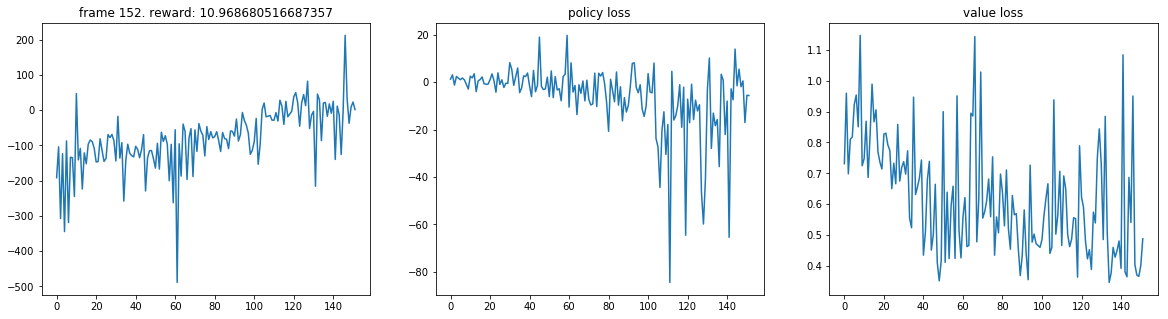
\includegraphics[height=0.41\textheight]{LunarLander-A2C-train}
    \caption{The reward, policy loss and value loss plots from training the A2C
             agent on the \texttt{LunarLander-v2} environment.}
    \label{ref:lunar-a2c-train}
   \end{figure}
 
   \begin{figure}
    \centering
    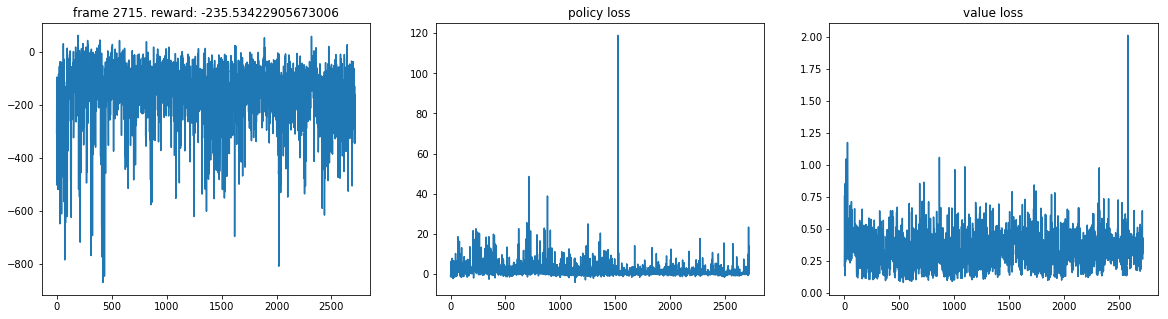
\includegraphics[height=0.41\textheight]{LunarLander-PPO-train}
    \caption{The reward, policy loss and value loss plots from training the PPO
             agent on the \texttt{LunarLander-v2} environment.}
    \label{fig:lunar-ppo-train}
   \end{figure}
  \end{landscape}

 \section[Performance comparison of A2C and PPO]{Performance comparison of 
   Advantage Actor Critic and Proximal Policy Optimization}
 %%%%%%%%%%%%%%%%%%%%%%%%%%%%%%%%%%%%%%%%%%%%%%%%%%%%%%%%%%%%%%%%%%%%%%%%%%%%%%%
  In this section we will be comparing the performance of A2C and PPO in 2
  different environments.

 \section[Analysis of A2C and PPO in different environments]{Analysis of 
   Advantage Actor Critic and Proximal Policy Optimization in different 
   environments}
 %%%%%%%%%%%%%%%%%%%%%%%%%%%%%%%%%%%%%%%%%%%%%%%%%%%%%%%%%%%%%%%%%%%%%%%%%%%%%%%
  In this section I will analyze the performance of A2C and PPO in two 
  different environments.

  \subsection[The \texttt{CartPole-v1} environment]{Performance analysis in the
    \texttt{CartPole-v1} environment}
  %%%%%%%%%%%%%%%%%%
   In this section I will compare the performance in the \texttt{CartPole-v1} 
   environment.

  \subsection[The \texttt{LunarLander-v2} environment]{Performance analysis in 
    the \texttt{LunarLander-v2} environment}
  %%%%%%%%%%%%%%%%%%
   In this section a comparison of the performance in the \texttt{LunarLander-v2} environment will be made.


%%%%%%%%%%%%%%%%%%%%%%%%%%%%%%%%%%%%%%%%%%%%%%%%%%%%%%%%%%%%%%%%%%%%%%%%%%%%%%%%


 \begin{thebibliography}{9}
  \bibitem{mets-policy-gradient}
   Kevin Mets, ``Policy Gradient Methods'', \textit{blackboard.uantwerpen.be}, 2020. [Online]. Available: \url{https://blackboard.uantwerpen.be/webapps/blackboard/execute/content/file?cmd=view&content_id=_2229370_1&course_id=_1892_1}. [Accessed: May 1, 2020].
  \bibitem{gym}
   OpenAI, ``Gym'', \textit{gym.openai.com}. [Online]. Available: \url{gym.openai.com}. [Accessed: May 1, 2020].
 \end{thebibliography}

%%%%%%%%%%%%%%%%%%%%%%%%%%%%%%%%%%%%%%%%%%%%%%%%%%%%%%%%%%%%%%%%%%%%%%%%%%%%%%%%

 \appendix

 \section{Jupyter Notebook for the \texttt{CartPole-v1} environment}
 \label{sec:cartpole-notebook}
 %%%%%%%%%%%%%%%%%%%%%%%%%%%%%%%%%%%%%%%%%%%%%%%%%%%%%%%%%%%%%%%%%%%%%%%%%%%%%%%
 \includepdf[pages=-]{CartPole/A2C_PPO.pdf}

 \section{Jupter Notebook for the \texttt{LunarLander-v2} environment}
 \label{sec:lunar-notebook}
 %%%%%%%%%%%%%%%%%%%%%%%%%%%%%%%%%%%%%%%%%%%%%%%%%%%%%%%%%%%%%%%%%%%%%%%%%%%%%%%
 \includepdf[pages=-]{LunarLander/A2C_PPO.pdf}

\end{document}
